\documentclass[10pt]{article}

\usepackage[margin=0.75in]{geometry}
\usepackage{times}
\usepackage[utf8]{inputenc}
\usepackage[T1]{fontenc}
\usepackage{booktabs}
\usepackage{amsfonts}
\usepackage{amsmath}
\usepackage{amssymb}
\usepackage{graphicx}
\usepackage{xcolor}
\usepackage{natbib}
\usepackage{url}
\def\UrlBreaks{\do\/\do-}
\usepackage{enumitem}
\setlist{nosep,leftmargin=*}

\definecolor{citecolor}{HTML}{0071BC}
\definecolor{linkcolor}{HTML}{0071BC}
\usepackage[pagebackref=false, breaklinks=true, colorlinks,
  citecolor=citecolor, linkcolor=linkcolor, bookmarks=false]{hyperref}

\newcommand{\method}{polynomial hint preconditioning}
\newcommand{\Method}{Polynomial hint preconditioning}

% Compact sections
\usepackage{titlesec}
\titlespacing*{\section}{0pt}{1.5ex plus 0.5ex minus 0.2ex}{0.8ex plus 0.2ex}
\titlespacing*{\subsection}{0pt}{1.0ex plus 0.3ex minus 0.1ex}{0.5ex plus 0.1ex}
\titlespacing*{\paragraph}{0pt}{0.6ex plus 0.2ex minus 0.1ex}{0.5em}
\titleformat*{\section}{\large\bfseries}
\titleformat*{\subsection}{\normalsize\bfseries}

% Compact captions and floats
\usepackage[font=small,labelfont=bf,skip=4pt]{caption}
\setlength{\textfloatsep}{8pt plus 2pt minus 2pt}
\setlength{\floatsep}{6pt plus 2pt minus 2pt}
\setlength{\intextsep}{6pt plus 2pt minus 2pt}
\setlength{\abovecaptionskip}{4pt}
\setlength{\belowcaptionskip}{2pt}

% Compact abstract
\renewenvironment{abstract}
  {\small\begin{center}\bfseries Abstract\end{center}\vspace{-0.5em}\begin{quote}\small}
  {\end{quote}\vspace{-0.5em}}

\title{\Large Polynomial Hint Preconditioning for\\Universal Time Series Forecasting}

\author{
  Anonymous
}

\date{}

\begin{document}

\maketitle
\vspace{-1.5em}

\begin{abstract}
Patch-based transformers for time series forecasting embed each patch independently, creating a cross-patch information bottleneck: temporal patterns spanning multiple patches must be recovered entirely through attention. We propose \textbf{polynomial hint preconditioning}, which applies a fixed Chebyshev FIR filter to the input and concatenates the result as an auxiliary channel before patching. This injects cross-patch temporal information with negligible overhead (12K parameters, 0.11\%). On GIFT-Eval (97 configurations, 5 seeds), our method improves geometric mean MASE by 2.9\% over the Moirai-2 Small baseline ($p < 10^{-15}$), winning 329/485 comparisons. Controlled ablations---duplicate channel \emph{hurts} (44.7\% wins), zero channel is neutral---confirm the improvement is driven by polynomial content. At 100K training steps, the benefit grows to 3.9\%.
\end{abstract}

%==============================================================================
\section{Introduction}
%==============================================================================

Universal time series forecasting models~\citep{woo2024unified,das2024decoder,ansari2024chronos} train on diverse corpora to generalize zero-shot. The Moirai family~\citep{woo2024unified,liu2024moirai2} uses patch-based transformer encoders: the input is split into non-overlapping patches of size $P$, each projected to a $d$-dimensional embedding~\citep{nie2023patchtst,dosovitskiy2021image}. This creates a \emph{cross-patch information bottleneck}: before the first attention layer, each embedding encodes only $P$ time steps, so multi-patch patterns (e.g., daily cycles in hourly data spanning 1.5 patches) must be discovered through attention alone.

We propose \textbf{polynomial hint preconditioning}: before patching, we apply a fixed Chebyshev polynomial FIR filter~\citep{oppenheim1999discrete,parks1972chebyshev} to the raw series and concatenate the result as an auxiliary input channel:
\begin{equation}
h[t] = T_d(B^s)\, x[t], \quad s = P,
\end{equation}
where $T_d$ is the degree-$d$ Chebyshev polynomial and $B^s$ is the backshift operator. For $d{=}4$, $s{=}16$: $h[t] = x[t] - 2x[t{-}32] + 0.5x[t{-}64]$, injecting information from 2 and 4 patches back. Only the input projection widens (12K extra parameters out of 11.4M). This is inspired by universal sequence preconditioning~\citep{marsden2024universal}, which shows polynomial transformations reduce spectral complexity for online prediction. We provide the filtered signal as a ``hint'' rather than replacing the input, letting the model combine both representations.

%==============================================================================
\section{Method}
%==============================================================================

\paragraph{Hint channel.} Given the normalized time series $x$, we compute the hint residual $\tilde{h}[t] = T_d(B^s)x[t] - x[t]$ and partition it into patches aligned with the original patching. The input to the projection becomes $3P$-dimensional: $\mathbf{e}_i = \text{ResBlock}_{3P \to d}([\mathbf{p}_i; \mathbf{m}_i; \tilde{\mathbf{h}}_i])$, where $\mathbf{p}_i$ is the data patch, $\mathbf{m}_i$ the observation mask, and $\tilde{\mathbf{h}}_i$ the hint patch. Only the first linear layer widens; the transformer encoder is unchanged.

\paragraph{Hint dropout.} During training, each patch's hint is independently zeroed with probability $p_{\text{drop}}{=}0.1$, preventing over-reliance on hints. At inference, the full hint is provided.

\begin{figure}[t]
\centering
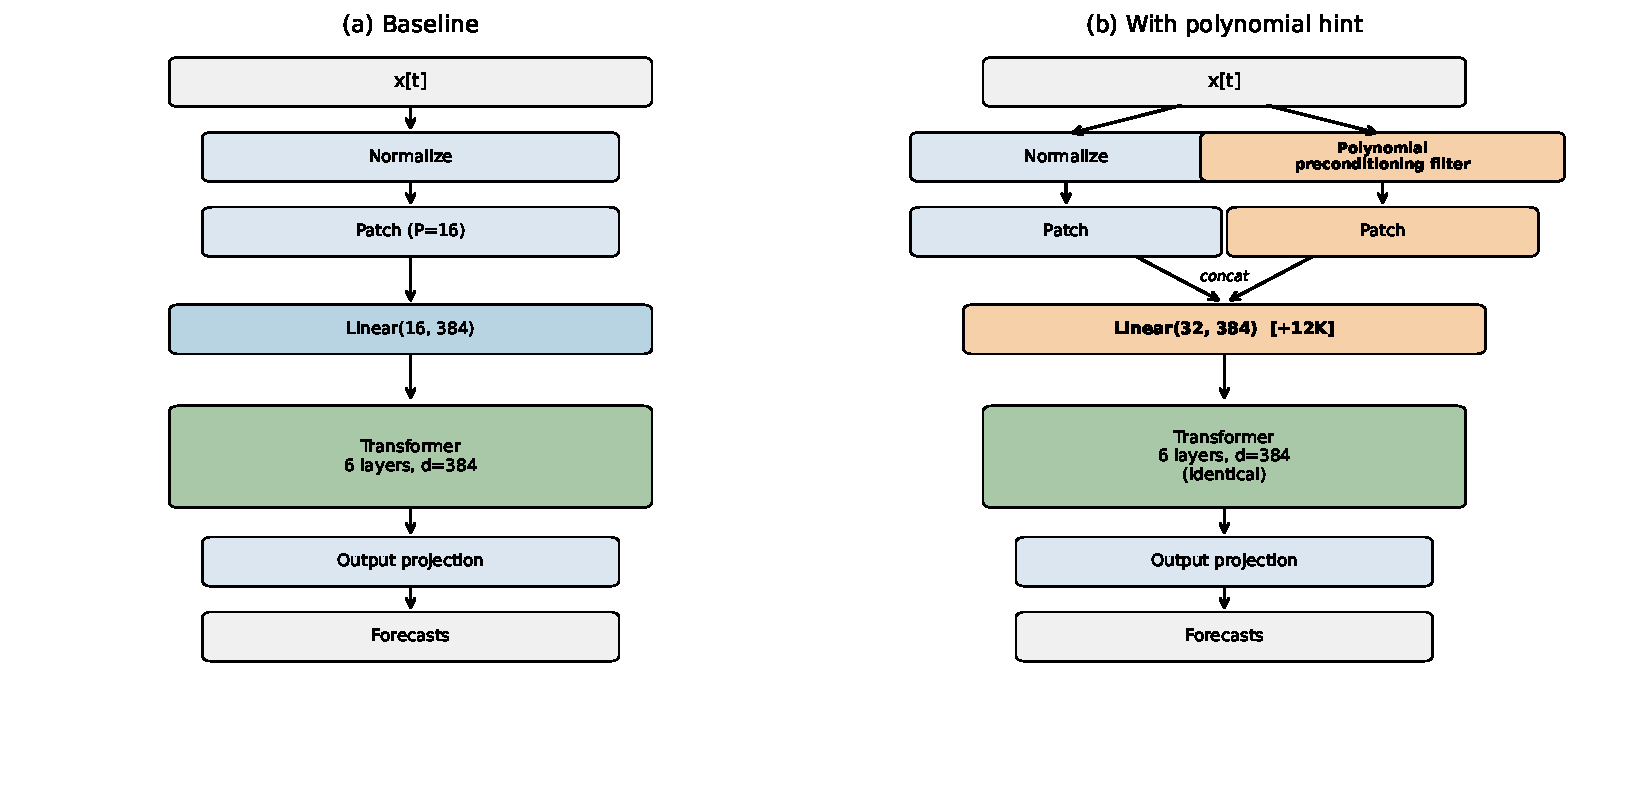
\includegraphics[width=\linewidth]{figures/fig_architecture.pdf}
\vspace{-1.5em}
\caption{Overview: (a) standard patch transformer; (b) with hint preconditioning. Only the input projection is wider (orange). Total overhead: 12K parameters (0.11\%).}
\label{fig:arch}
\vspace{-0.5em}
\end{figure}

%==============================================================================
\section{Experiments}
%==============================================================================

\paragraph{Setup.} We train Moirai-2 Small~\citep{liu2024moirai2} (11.4M params, 6-layer transformer, $P{=}16$) from scratch on the LOTSA corpus~\citep{woo2024unified} for 10K steps (batch 256, AdamW, cosine LR $10^{-3}$, 1K warmup, bf16). Evaluation uses GIFT-Eval~\citep{vijay2024gifteval} (97 dataset$\times$horizon configs) with geometric mean MASE at context length 4,000. We run 5 seeds (0, 1, 2, 7, 42) and use paired sign tests pooled across seeds (485 comparisons).

\paragraph{Conditions.} Baseline (standard Moirai-2), Zero (hint architecture with all-zero hints), Duplicate (hint = copy of input), and \textbf{HD10} (Chebyshev $d{=}4$, stride 16, 10\% dropout).

\subsection{Main Results}

\begin{table}[t]
\centering
\caption{Main results (5 seeds, 485 comparisons on GIFT-Eval). HD10 significantly outperforms baseline and both capacity controls.}
\label{tab:main}
\small
\begin{tabular}{lcccc}
\toprule
\textbf{Method} & \textbf{Mean MASE} & \textbf{vs BL} & \textbf{Wins/485} & \textbf{$p$-value} \\
\midrule
\textbf{HD10 (Ours)} & \textbf{1.1765} & \textbf{$-$2.89\%} & \textbf{329 (67.8\%)} & $\mathbf{1.5 \times 10^{-15}}$ \\
Zero channel & 1.2061 & $-$0.45\% & 262 (54.0\%) & 0.042 \\
Baseline & 1.2116 & --- & --- & --- \\
Duplicate channel & 1.2162 & $+$0.38\% & 217 (44.7\%) & 0.99 \\
\bottomrule
\end{tabular}
\vspace{-0.5em}
\end{table}

Table~\ref{tab:main} shows that HD10 improves MASE by 2.9\% over the baseline ($p < 10^{-15}$). The capacity controls confirm the polynomial content drives the improvement: a \emph{duplicate} channel hurts (44.7\% wins), while a \emph{zero} channel is neutral (54.0\%). HD10 vs.\ Duplicate: 336/485 wins ($p = 6 \times 10^{-18}$). HD10 wins on every seed individually (range: $+0.4\%$ to $+5.0\%$).

\subsection{Ablations}

\begin{figure}[t]
\centering
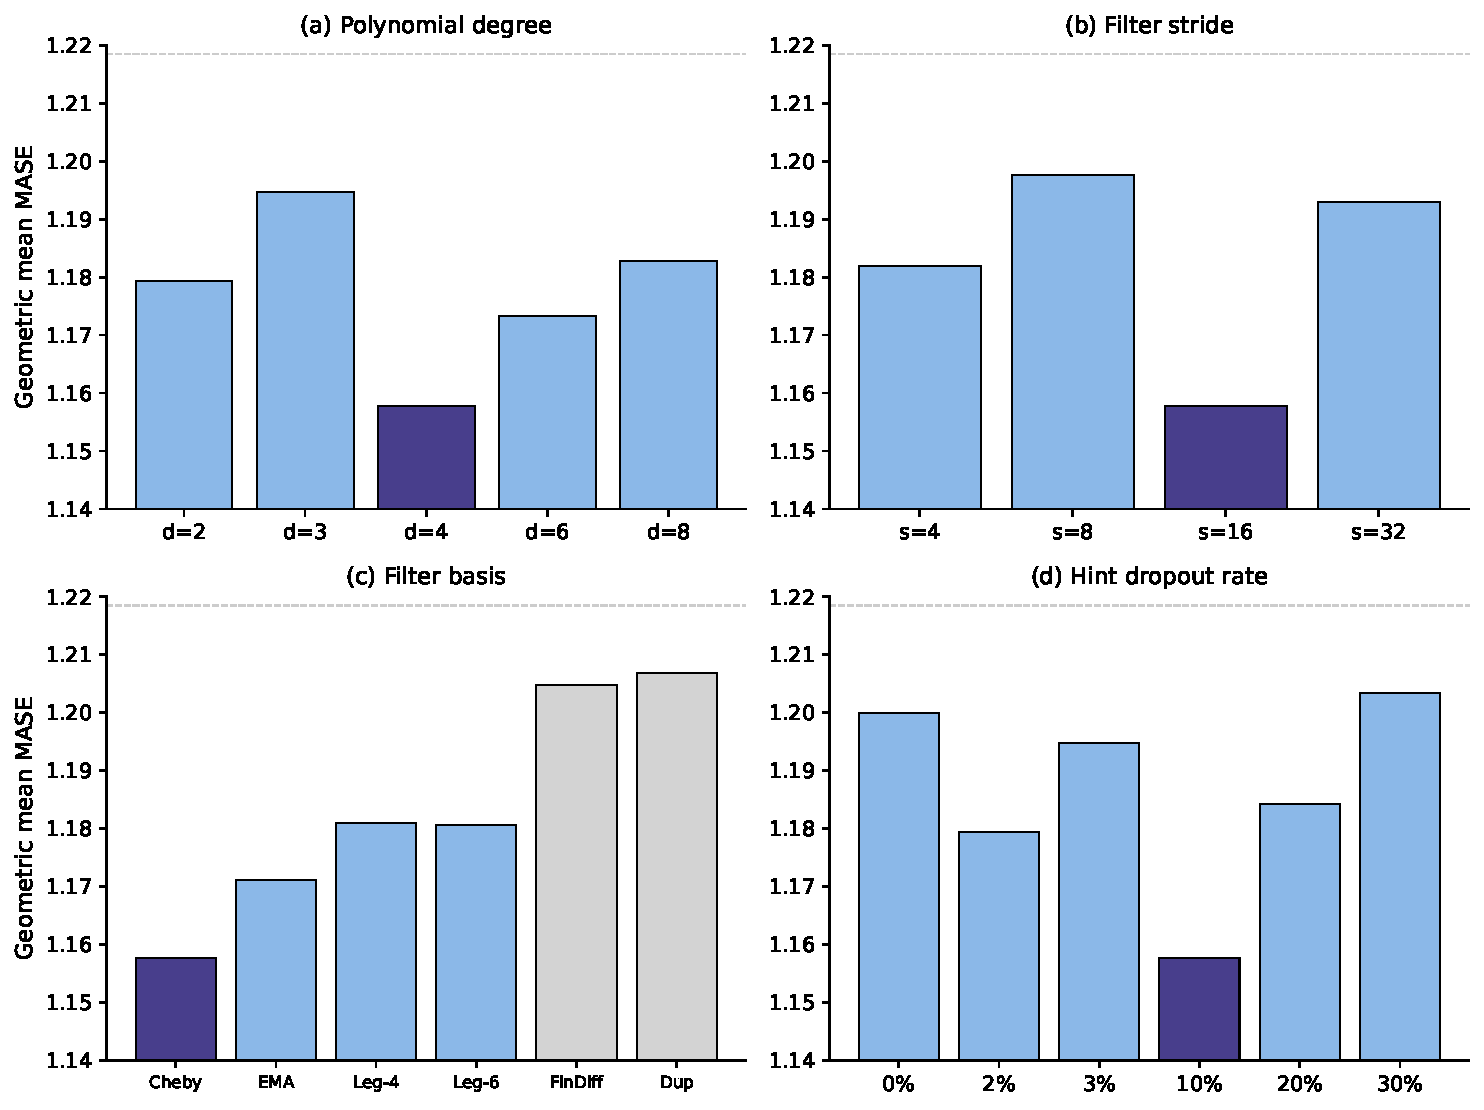
\includegraphics[width=\linewidth]{figures/fig2_ablations.pdf}
\vspace{-1.5em}
\caption{Ablations (seed 0, 97 configs). Bar labels: wins/97 vs.\ baseline. Dashed line: baseline. Orange: optimal. (a) Degree $d{=}4$ optimal. (b) Stride $s{=}16{=}P$ optimal. (c) Chebyshev basis best. (d) 10\% hint dropout optimal.}
\label{fig:ablations}
\vspace{-0.5em}
\end{figure}

Figure~\ref{fig:ablations} summarizes ablations over polynomial degree ($d{=}4$ optimal), filter stride ($s{=}P$ optimal---filter taps align with patch boundaries), basis type (Chebyshev $>$ EMA $>$ Legendre $\gg$ finite differences), and hint dropout (10\% optimal, inverted-U pattern). An inference-time ablation confirms the model learns specific polynomial structure: replacing hints with zeros degrades MASE by 9.3\%; random noise by 14.5\%; duplicate input by 29.9\%.

\subsection{Extended Training and Analysis}

At 100K training steps (5 seeds), HD10 improves by 3.9\% over the baseline (mean MASE 1.1871 vs.\ 1.2351), while Duplicate ($-0.9\%$) and Zero ($-1.7\%$) both \emph{hurt}. The baseline exhibits training instability at long horizons (seed variance 1.21--1.28), while HD10 stays stable (1.17--1.21). Notably, training loss differences are much smaller than eval gains: at 10K steps, HD10's loss is only 1.0\% lower than baseline (0.1350 vs.\ 0.1364), yet eval MASE improves by 2.9\%---a $2.9\times$ amplification ($2.4\%$ vs.\ $3.9\%$ at 100K). Duplicate and Zero controls have training loss comparable to baseline despite worse eval, confirming that hints act as a regularizer rather than an optimization accelerator.

\paragraph{Domain \& frequency.} The benefit is strongest in high-frequency domains: transport ($+6.9\%$, $p{=}4{\times}10^{-8}$), energy ($+4.0\%$, $p{=}2{\times}10^{-4}$), consistent with the filter's lookback scale (32, 64 steps = 8, 16 hours for 15-min data). Weather and healthcare show no significant improvement. The benefit increases with prediction horizon ($+1.4\%$ short $\to$ $+5.1\%$ long) and is approximately constant (${\sim}5\%$) across context lengths 512--4,000. HD10 at context 2,000 outperforms the baseline at context 4,000 (1.1713 vs.\ 1.2185).

\paragraph{Learning rate robustness.} HD10 is insensitive to learning rate (0.1\% difference between $\eta{=}10^{-3}$ and $2{\times}10^{-3}$), while the baseline varies by 2.3\%. At matched optimal LR ($2{\times}10^{-3}$), HD10 still wins significantly (280/485, $p{=}3.8{\times}10^{-4}$), though the effect is smaller ($+0.7\%$).

%==============================================================================
\section{Related Work}
%==============================================================================

Time series foundation models~\citep{woo2024unified,liu2024moirai2,das2024decoder,ansari2024chronos,goswami2024moment} train on large corpora for zero-shot forecasting. Patch-based architectures~\citep{nie2023patchtst,dosovitskiy2021image} are now dominant, with PatchTST using overlapping patches to partially address the cross-patch bottleneck. Our approach is orthogonal: we inject cross-patch information via a fixed filter with no change to attention. The polynomial basis is motivated by universal sequence preconditioning~\citep{marsden2024universal}, which provides theoretical guarantees for polynomial transformations in online prediction, building on spectral filtering~\citep{hazan2017learning,hazan2018spectral}. FIR filter design with Chebyshev polynomials is classical~\citep{parks1972chebyshev,oppenheim1999discrete}.

%==============================================================================
\section{Conclusion}
%==============================================================================

Polynomial hint preconditioning adds a fixed Chebyshev FIR-filtered channel to patch-based time series transformers, injecting cross-patch temporal information at 0.11\% parameter overhead. On GIFT-Eval with 5 seeds, it improves MASE by 2.9\% ($p < 10^{-15}$), with controlled ablations confirming the polynomial content---not extra capacity---drives the gain. The method is applicable to any patch-based architecture~\citep{woo2024unified,nie2023patchtst,das2024decoder} with no modification to the transformer encoder. Limitations include reduced benefit at matched optimal learning rate ($+0.7\%$), no improvement on weather/healthcare domains, and inconsistent results at larger model scales (46M parameters).

\bibliography{references}
\bibliographystyle{plainnat}

\end{document}
